\item \points{3b} \textbf{Coding problem: vanilla logistic regression}

First, we use the vanilla logistic regression to learn an imbalanced dataset. For the rest of the question, we will use the dataset and starter code provided in
the following files:
%
\begin{center}
	\begin{itemize}
		\item	\texttt{src-imbalanced/{train,validation}.csv}
		\item   \texttt{src-imbalanced/submission.py}
	\end{itemize}
\end{center}

Please complete |apply_logistic_regression| and |calculate_accuracies| functions.

Each file contains $n$ examples, one example $(x^{(i)}, y^{(i)})$ per row. $x$ is two-dimensional, i.e., the $i$-th row contains columns $x^{(i)}_1\in\Re$,
$x^{(i)}_2\in\Re$, and $y^{(i)}\in\{0, 1\}$. Let $\calD=\{(x^{(i)}, y^{(i)})\}_{i=1}^n$ be our training dataset. $\calD$ has $\rho n$ examples with label 1 and $(1-\rho)n$ with label 0. In the dataset we constructed, $\rho=1/11$.

You will train a linear classifier $h_{\theta}(x)$ with average empirical loss for logistical regression, where $h_\theta(x)=g(\theta^T x), g(z)=1/(1+e^{-z})$, similar to Problem 1 Part a:
\begin{align*}
J(\theta) = -\frac{1}{\nexp} \sum_{i=1}^\nexp \left(y^{(i)}\log(h_{\theta}(x^{(i)}))
+  (1 - y^{(i)})\log(1 - h_{\theta}(x^{(i)}))\right), 
\end{align*}

After obtaining the classifier, compute the classifier's accuracy ($A$), balanced accuracy ($\overline{A}$), accuracies for the two classes ($A_0, A_1$) on the validation dataset. You are expected to observe that the minority class (positive class) has significantly lower accuracy than the majority class. 

The output plot should look similar to the following (no plot submission is required):

\begin{figure}[H]
	\centering
	\vspace{2mm}
	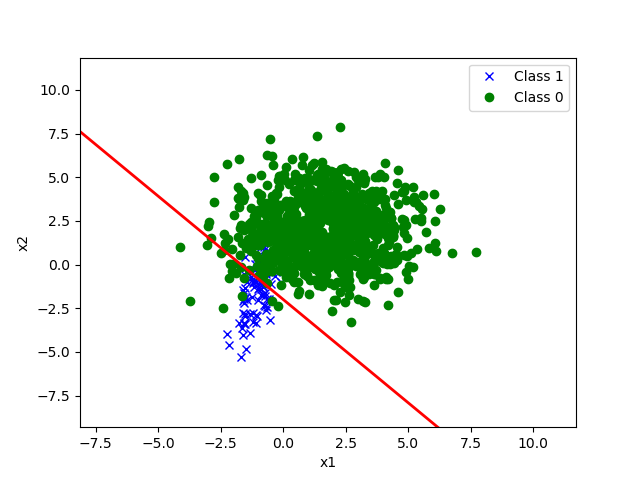
\includegraphics[width=0.5\linewidth]{03-imbalanced/imbalanced_naive_pred.png}
	  \caption{Validation set with $x_1$ on the horizontal axis and $x_2$ on
	  the vertical axis. The decision boundary obtained by your model (i.e, line corresponding to model's predicted probability = 0.5).}
  \end{figure}
